
\section{Implementation Issues}
\label{sec:implementation}

Although a completed and detailed floorplan of the node is not the
focus of this work, in this section we want to give a basic idea of
which are the main elements required to support this kind of
architecture thus giving an estimate of the overhead by the
DiSR approach. There are three main classes of node elements:
\begin{itemize}
\item Node-specific: components (such ALUs, memories) that are
strictly related to the node functionality and role inside a given
network, e.g. being a computation or storage node.
\item Node communication:  these are elements (such as transceivers,
buffers) required to the node to communicate with its neighbours,
independently from node functionality and DiSR implementatio
\item DiSR-specific: all the hardware, control logic and
configuration registers, related to an implementation the proposed approach.
\end{itemize}

\begin{figure}
  \centering
  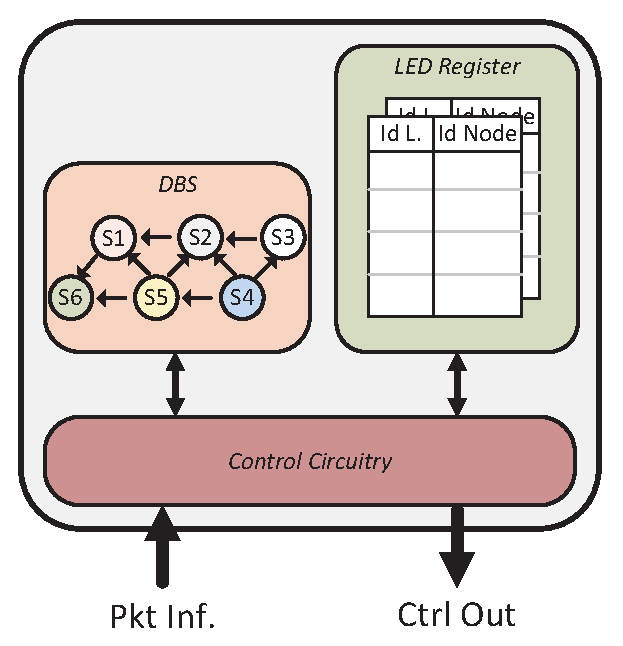
\includegraphics[width=0.25\textwidth]{pictures/disr_imp.eps}
  \caption{\emph{DiSR} block architecture.}
 \label{fig:implementation}
\end{figure}

Let's so focus to the \emph{DiSR} block. In
Fig.~\ref{fig:implementation} is shown a possible sketch of this
block, which mainly consist in the following building elements:

\begin{itemize}
\item \emph{DBS block}: It Takes trace of the DBS, and how already
discussed in the Section~\ref{ssec:disr_dstruct}, there are six possible
configurations. These values can be codified using 3 bit implemented
with a 3-bit register and the required combinational logic. This block
is essentially designed as a state machine.
\item \emph{LED registers}: Is a set of registers useful for storing
the local environment data (LED) described in
Section~\ref{ssec:disr_dstruct}. In particular in
fig.~\ref{fig:implementation}, are highlighted two tables representing
the \emph{link\_visited[]} and \emph{link\_tvisited[]} values. This
block consists of an array of registers (one for each
direction) that can be implemented with an SRAM, in which are presents
two specific fields  for representing the \emph{segID}. 
\item \emph{Control circuitry}: This circuitry reads data
from the fields of the incoming packet, LED registers and the
\emph{DBS}, updating \emph{LED} and
\emph{DBS} data when required. Then, the resulting \emph{Ctrl Out} output  drives the other
communication resources (such as node transceivers) for actuating the
DiSR routing operation.
\end{itemize}

As discussed above, one of the main design challenge of DNA
Self-Assembled systems is the limited resource available for
implementing both computations and routing decisions for each node.
For this reason, assuming a budget of $10^4$ CNFETs for each network's
node~\cite{liu_jetcs} we estimated the required resource for
implementing the entire DiSR block. A not optimized behavioural
HDL of the DiSR circuitry has been written and synthesized at gate-level.
Considering the specific layout of each single logic elements ( NAND,
full-adder, latch etc.), it has been possible to get a rough estimate
of the number of transistors necessary for implementing the DiSR
logic.  Figure~\ref{fig:imp_trend} shows the results of synthesis in
terms of number of devices (CNFETs) versus the number of network nodes
while the network scales up from $10\times10$ to $100\times100$ nodes.
\begin{figure}
  \centering
  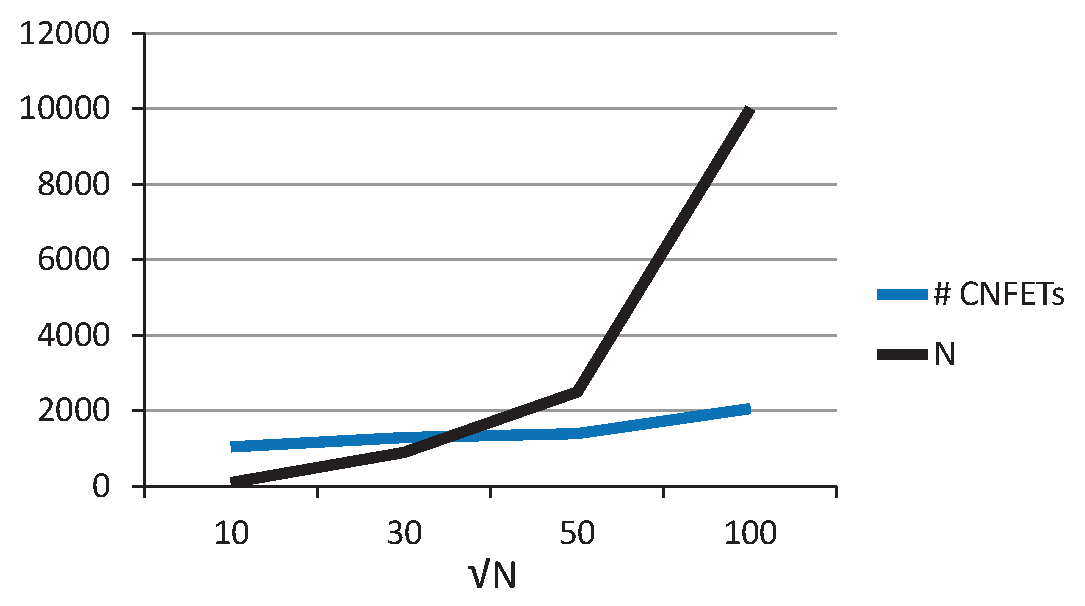
\includegraphics[width=0.25\textwidth]{pictures/imp_rslt.eps}
  \caption{DiSR synthesis results: N is the number of network's node.}
 \label{fig:imp_trend}
\end{figure}
In particular, observing the Fig.\ref{fig:imp_trend} can 
be pointed out that the proposed implementation occupy  about 20\% of the node budget. 
Further, more than the absolute number of devices itself, it is interesting to
observe that, while the node have a squared increment, the circuitry
complexity which implements the DiSR algorithm increases with a slowly
growing trend.  
An intuitive explanation of this is the relatively simple logic of
DiSR, whose behaviour is almost code on scalable storage structures.
For example, the number of registers implementing the
\emph{link\_visited[]} and \emph{link\_tvisited[]} table follow the
logarithmic function:
\begin{equation}
  \label{eq:imp_trend}
  N_{reg}=2\cdot N_{port} \cdot log_2(N)
\end{equation}
where $N_{port}$ is the number of the router's ports, $N$ is the number 
of network's nodes while the term $2$ takes in account that \emph{link\_visited[]} and 
\emph{link\_tvisited[]} are two separate set of registers. While this number is fixed by 
the number of network's node, the control circuitry could be optimized applying more effort 
in future designs of this building block. 

